\chapter{Introduction}

The term network system passes on, an association of various PCs. For the most part, these systems have two kinds of availability, which are wired and remote. As on account of any innovation, it is development came out as a need. For any country, its most extreme need is to keep up military certainty. During the change from the electrical and mechanical age to the electronic age, everything from regular family unit things to bank the board experienced a significant overhaul. Normally, this implied the safeguarded area grasped innovation sometime before. The entire first network system was essential and was set up in a military resistance venture called ARPANET, representing the Advanced Research Projects Agency Network. It was the beginning stage of the current web. PC arranges throughout the years have developed a wide margin regarding highlights, intricacy, and power. That as well as it has extended its scope to the business and new parts. In these advanced occasions, terms such as switches and passages, are recognizable to even the layman.
\vspace{5mm}
\section{Traditional Networks}

Even something as new and intense as network systems have demonstrated age. The maturing of innovation is by all accounts a lot snappier than people. Inside two decades, it built up an area of systems classified as traditional networks. Traditional networks are the spearheading plan of networks. Adam Smith of computer networking had a structure that was solid for the time and had no issues for quite a while. Indeed, even today, the traditional network system engineering cannot be blamed as is yet a subject of innovative work. Nevertheless, concerning each innovation that exists, there will be advantages and disadvantages.

\begin{figure}[!hbt]
    \centering
    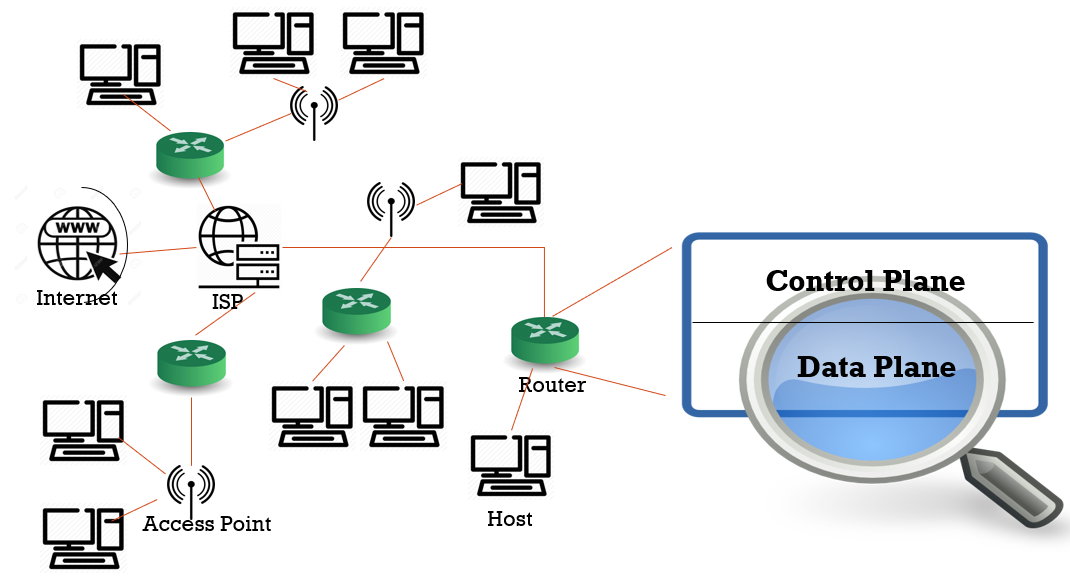
\includegraphics[width=\textwidth,keepaspectratio]{images/TRADITIONAL-NETWORK.png}
    \caption{Traditional Networks \cite{sdnimages}}
    \label{fig:Tradnets}
\end{figure}

   The computer network was developed for the sole purpose of communication. So this meant carrying digital information from one machine to another remote machine, via wire or air. It is similar to the case of sending a post from one individual to another. A post was given to the post office, which redirects it to another post office, which would be closest to the receiver's address.
    
    This task of forwarding the post is the same in the case of computer networks and termed as routing. In computer networks, no humans are interfering; rather, there are individual devices in charge of performing this data forwarding. The task of routing is delegated to devices called routers, which make up a fair share of the entire global network today.
    
    Routers play the most crucial role in today's network, i.e., forwarding packets via specific routes by figuring out the current situation of the neighboring network devices and keeping track of the connected devices. Similar to how everybody has a PO box attached to their address, every device in a local network is registered under a router. These routers are scattered throughout the network and are necessarily the backbone of the network. The same reason is why this technique has been researched for years so that it has good fault tolerance and error correction. Such a network where there are millions of packet forwarding devices ensures redundancy, and as there is no single point of vulnerability.
    \vspace{2mm}
    
    This technique of routing has been used for a long time. It will continue to be used throughout the lifetime of computer networks. Over time, the techniques of routing have changed drastically, and different algorithms and network topologies \cite{topograph1996} have been researched and put forward, which makes computer networks much more efficient in modern times. However, just because something works well does not mean it cannot be improved. While the discussion is not about improving routing techniques, specifically, it is emphasized that the perception of computer networks seems too dull and obsolete. The concept of sending off a data packet with a header attached to it into the vast complexities of the worldwide web seems like tying a note to a carrier pigeon and sending it to fly. Yes, the pigeon knows how to reach the destination by a step-by-step process, but neither the sender nor the receiver nor the network administrator knows where the packet is until it reaches an informal network where either the recipient or the network administrator is continuously monitoring and waiting for the packet to arrive.
    
    Packet forwarding is one part of the network's function. Other features include monitoring the network and checking which routes are available and which routes are down or under huge loads so that the network traffic can be redirected to another route. Traditional networks have many well-known workarounds to such problems; many of them are clumsy and exploit the assumption that networking devices are capable of fast processing. They can handle many faults simultaneously without much effort. While this may be true, it opens a door for improvement. As of now, there is no central monitor to analyze a vast network's health. The individual routers and access points take checks on their immediate neighbors and assume their neighbors will do the same. It was a splendid thought at the time, but it seems too easy.
        
    Another criterion of traditional networks is that each protocol, network topology or architecture, assumes that the entire network would run a single protocol for a lifetime. Alternatively, in other words, no protocol considered the need for adaptability or compatibility for change depending on the scenario. Some protocols would adapt itself to handle network anomalies and maintain consistent and predictable performance. However, the concept of making a network that could change its hardware and software at any given time was far-fetched.
    
   In the case of network faults, there are many measures deployed to back up and make sure the network can be brought back up and running. However, the realization of network fault over the entire network is too slow in terms of computing speeds. If one router or a server fails somewhere in this vast network, the error message from its neighbors needs some time for it to get spread out and diffused to every other device in the network. This delayed response in the case of network faults is something that can be improved.
        
\section{Software Defined Networks}
    
    Traditional networks follow hardware-dependent software architecture. In other words, the networking devices used, for example, a router, came from a specific vendor, and the vendor uses either their own proprietary software on it or a third party software custom-made for their hardware. Instead, take the case of a personal computer. It has hardware made from a vendor, but the hardware design allows us to install any operating system on it and use the computer in any means. Obviously, some operating systems offer more or better features than some others.
    
     The entire network has a hardware platform which suitable for any or multiple operating systems at a time. The entire network is not defined by the hardware, instead of the operating system that runs on it and manages the network.
    
    Such an architecture is implemented by taking a centralized network approach on decentralized network architecture. The sentence sounds like an oxymoron, but the gist of it is to extend the decentralized network architecture by maintaining the data forwarding methods in its place and collectively centralizing the network decision-making processes into a logically single entity. In other words, the routing functionality from the routers are removed, and they behave as switches while making a central entity to perform the routing decisions and monitor the entire network. This entity is termed as ''Controller''. This thesis mainly focuses on controllers and the server where it is installed.
    
\begin{figure}[!hbt]
    \centering
     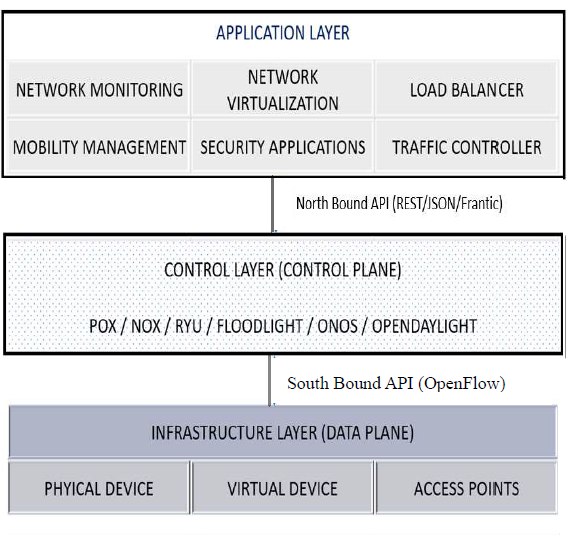
\includegraphics[width=\textwidth,keepaspectratio]{images/SDN-architecture-example.png}
    \caption{SDN Architecture \cite{sdnimages}}
    \label{fig:SDN Architecure}
\end{figure}
    
    As described above, the software-defined network follows a divide and conquer approach to networking \cite{taxonomy2014}. Instead of making each and every router in the network to perform both the tasks of finding an optimal route to the destination, storing it to its own 'routing table' for future reference and notifying its neighbors of the change and at the same time, forwarding data packets of other predefined routes, it is load has been reduced and made to solely focus on data forwarding, by looking at a 'flow table' rather than calculating a route and updating it. In case it needs a new route, or if any predefined routes get obsolete, it merely pings the controller and complies.
    
     The controller performs all the functions of calculating routes, monitoring network topology, and checking network health. This provides a centralized interface to manage the entire network. The benefit of such a system is that there is no need to communicate the status of the network to the entire network. Instead, simply dump all information onto a central device or a collectively operating set of devices, and it will make sure that the network runs smoothly and in the most hassle-free manner.
     
    Another advantage of using a separate entity for controlling the network is that it allows the network to be protocol independent. In other words, the operating system or the software that is running on the controller is not fixed. The software-defined network architecture allows us to change the operating system whenever required \cite{arpanet2004}. Granted, it will be a time-consuming task before the network is up and running again, but it certainly is a quicker and cheaper alternative to having to change the software on all the devices in the network.

    In any technology, the rewards will always come at either a trade-off or at risk. From slow but convenient transportation of the bicycle to the spectacular but risky aviation technologies, development always comes at a cost.
    Similarly, in software-defined networking as well, there are some bills to be paid.
    
    Firstly the implementation of a collective entity called the controller is in the way of putting all eggs in one basket. This method, however efficient, still poses a risk. The general principle in any management technology is to increase redundancy. If, for a sizeable software-defined network, there is a single controller, in case of any faults ranging from power outages to natural disasters can cause the entire network to fail.  
    
    Another downside of software-defined networking is that the central controller does not necessarily monitor the actual traffic itself rather only the network's health and different routes. It does not necessarily monitor the traffic is because controllers are capable of monitoring network traffic using third-party applications. It is physically possible for the controller to continuously ping a switch in order to get the packets it handles and read its contents. However, it is incredibly impractical, and therefore pursuing such a feature would yield fewer returns than the effort put in. So naturally, developers do not focus on traffic monitoring as much as compared to network monitoring and routing. This significantly reduces the scope of software-defined networking as networks in which traffic cannot be monitored efficiently would pose a risk in terms of authenticity and privacy. Unless the entire network is trusted by the network administrator and the network participants, such a method would seem less preferred.
    
    Last but not least, as an extension to the points prior to the previous one, since a single entity controls the entire network's routing and monitors the network health and topology, this will obviously result in a severe overhead on the controller. It was mentioned that software-defined networks are operating system independent, but they are, in a way, dependent on the hardware limitations. Such as processing power, network bandwidth, and will prevent the network from growing beyond an absolute scale. As the network scales, so does the complexity in handling such an extensive network. Tasks such as routing, topology discovery \cite{netflow2004} become cumbersome unless the controller hardware is upgraded.
    
    Also, this makes the network elastic, meaning it tends to want to return to its original dimensions, due to overstress on the controller. Unless the controller device is changed, which, although not that expensive or time-consuming, generates a degree of unreliability in the network, in traditional networks, load balancing on routes would be performed by neighboring routers, and the task of network monitoring was delegated, this meant that the network overhead would never go beyond a limit. In case all the routers in the network reached its limit, merely adding more routers and breaking down large networks to smaller subnets would be enough. However, that is uncertain in the case of software-defined networks. Distributed controllers solve this problem to an extent, but still need more time to develop into a more robust approach.
    
    \section{Motivation \& Problem Statement}
    
    Software-Defined Networks brings a new perspective to network architectures. The concept of having a centralized approach to decentralized network architecture brings the merits of both architectures.  SDN architecture provides the infrastructural flexibility and robustness of the traditional networks with the added feature of having a central interface to monitor and manage the entire network.
    
    There are many SDN implementations, each with a different controller operating system. However, there comes a question to choose the suitable controller for a network scenario where there are limited resources. Here, controllers are analyzed and tested for system-level performance metrics under a massive network traffic that appears similar to real-world networks. It helps to identify system-level bottlenecks of the controllers and makes it possible to classify controllers based on their system performances. It also generates the idea of whether the provided system is suited to a given controller and vice-versa.